\section{Webapp}
\subsection{Introduzione}
Rendere disponibili agli utenti finali i dati ottenuti dai servizi sopra presentati è responsabilità di una apposita applicazione web. 

Questa dovrà interfacciarsi con i vari middleware attraverso le API disponibili, per ottenere i dati da presentare all'utente in maniera il più possibile pratica e ordinata.

La web app sarà accessibile da browser e dovrà supportare anche dispositivi mobili, quindi reagire in maniera \textit{responsive} a schermi di dimensioni molto diverse. 


\subsection{Tecnologie utilizzate}
Essendo già a conoscenza dell'ambiente finale di deployment, la scelta delle tecnologie è stata presa top-down, per assicurare completa compatibilità e supporto.

La piattaforma Azure mette a disposizione diverse opzioni per l'hosting di una web app, che può essere ad esempio ospitata su una tradizionale macchina virtuale o come container app.

Le esigenze del nostro servizio dal punto di vista dell'interfaccia utente sono modeste, in quanto si tratta di una semplice vetrina per le informazioni disponibili, senza bisogno di autenticazione o salvataggio di dati in uno storage dedicato.

Delinandosi come applicazione prettamente front-end, la scelta è ricaduta su una Static Web App. Questo servizio Azure è pensato per ospitare web app full-stack che non hanno un tradizionale backend, e offre un supporto integrato ad API sotto forma di Azure Functions o Container App.

Le SWA sono costruite usando framework web come Angular, React o Vue, tecnologie per cui non è richiesto rendering lato server: le applicazioni sono costituite interamente da asset statici e file html/css/javascript. Questi sono serviti non da un web server tradizionale, bensì gestiti da Azure e distribuiti globalmente.

Il deployment delle nuove versioni avviene in maniera automatica a partire da cambiamenti in una repository di codice, come GitHub mediante \textit{Actions} o Azure stesso grazie alla \textit{DevOps Pipeline}. 
Il workflow è auto-generato da Azure e necessita pochi parametri di configurazione oltre alla repository (ed eventualmente branch) di riferimento. Questo modus operandi è, per design, molto vicino al flusso di lavoro tipico dello sviluppatore e permette uno sviluppo organico seguendo la pratica del \textit{Continuous Integration / Continuous Delivery}.

La scelta del framework javascript è ricaduta su Angular, sviluppato da Google e arrivato a luglio 2024 alla versione 18. È un framework open source maturo e facile da usare, adatto ad applicazioni web multipiattaforma.
È direttamente supportato da Azure Static Web Apps e rispetta la caratteristica richiesta di rendering lato browser.


\subsection{Angular}
Le app Angular sono scritte in typescript e devono seguire una precisa struttura. Sono \textit{single-page-applications} organizzate per componenti con singola responsabilità, componibili all'interno di file \texttt{.html} estesi per supportare tag aggiuntivi.

I componenti sono definibili direttamente in un unico file typescript ed esportati come classi. Sono identificati da un selettore, reso poi disponibile sotto forma di tag, e devono presentare un template HTML per istruire il rendering, che può anche essere inserito sotto forma di link a un file a sé.

È costume velocizzare lo sviluppo delle applicazioni web affidandosi a librerie di terze parti aggiuntive che mettano a disposizione componenti pronti all'uso. Nel caso di Courtsight è stato scelta \textbf{PrimeNG}.
Questa libreria molto completa è sviluppata da PrimeTek, che l'ha declinata per tutti i maggiori framework. Alla base di queste diverse librerie c'è il loro sistema \textit{PrimeFlex}, che permette una facile gestione della distribuzione dei componenti a schermo semplificando le direttive CSS "flex".

\subsection{Contenuto webapp}
    \paragraph{Homepage} La pagina principale del sito presenta all'utente i vari sport supportati. L'integrazione con la \texttt{bet\_api} ci può permettere in un futuro di mostrare le quote anche per sport diversi dal basket americano, che per ora rappresenta il principale focus.
    
    \begin{figure}[H]
        \centering
        \fbox{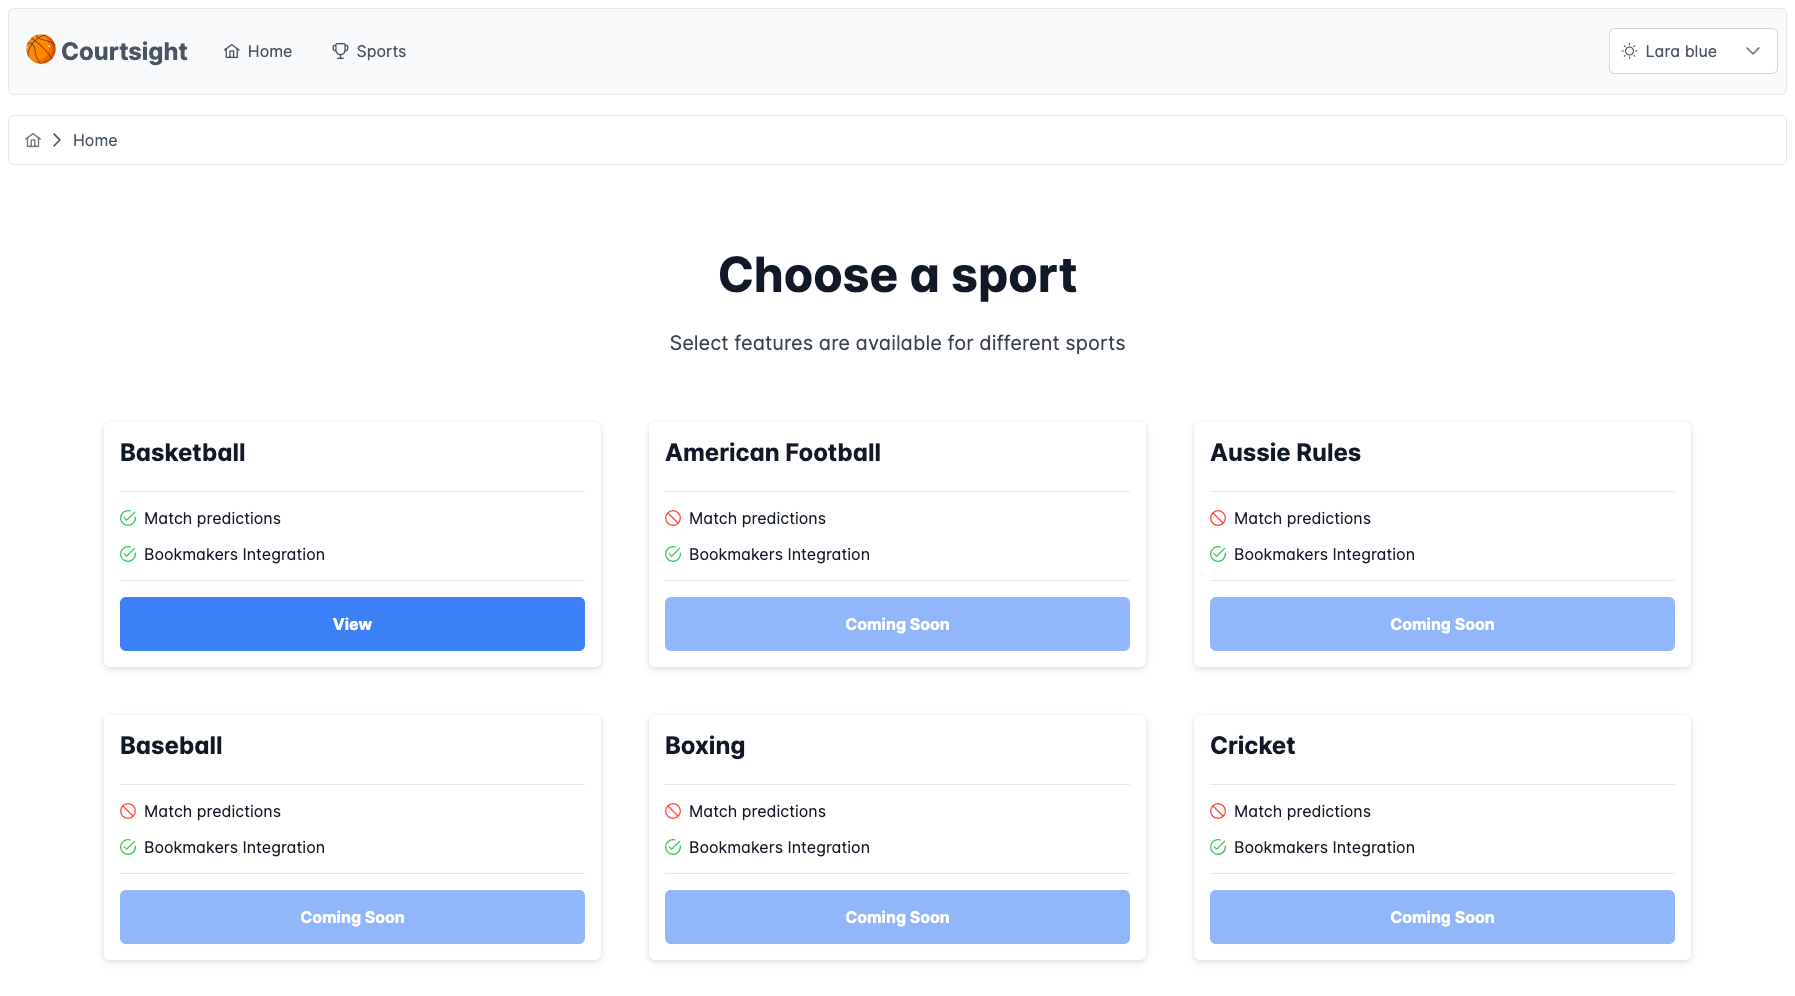
\includegraphics[width=0.75\linewidth]{img/webapp/homepage.png}}
        \caption{Homepage}
        \label{fig:enter-label}
    \end{figure}
    
    \paragraph{Home - Basket} La schermata home della sezione basket offre l'elenco delle partite della settimana attuale e la classifica aggiornata al periodo esposto, divisa tra le due conference NBA: East e West Coast. 
    \begin{figure}[H]
        \centering
        \fbox{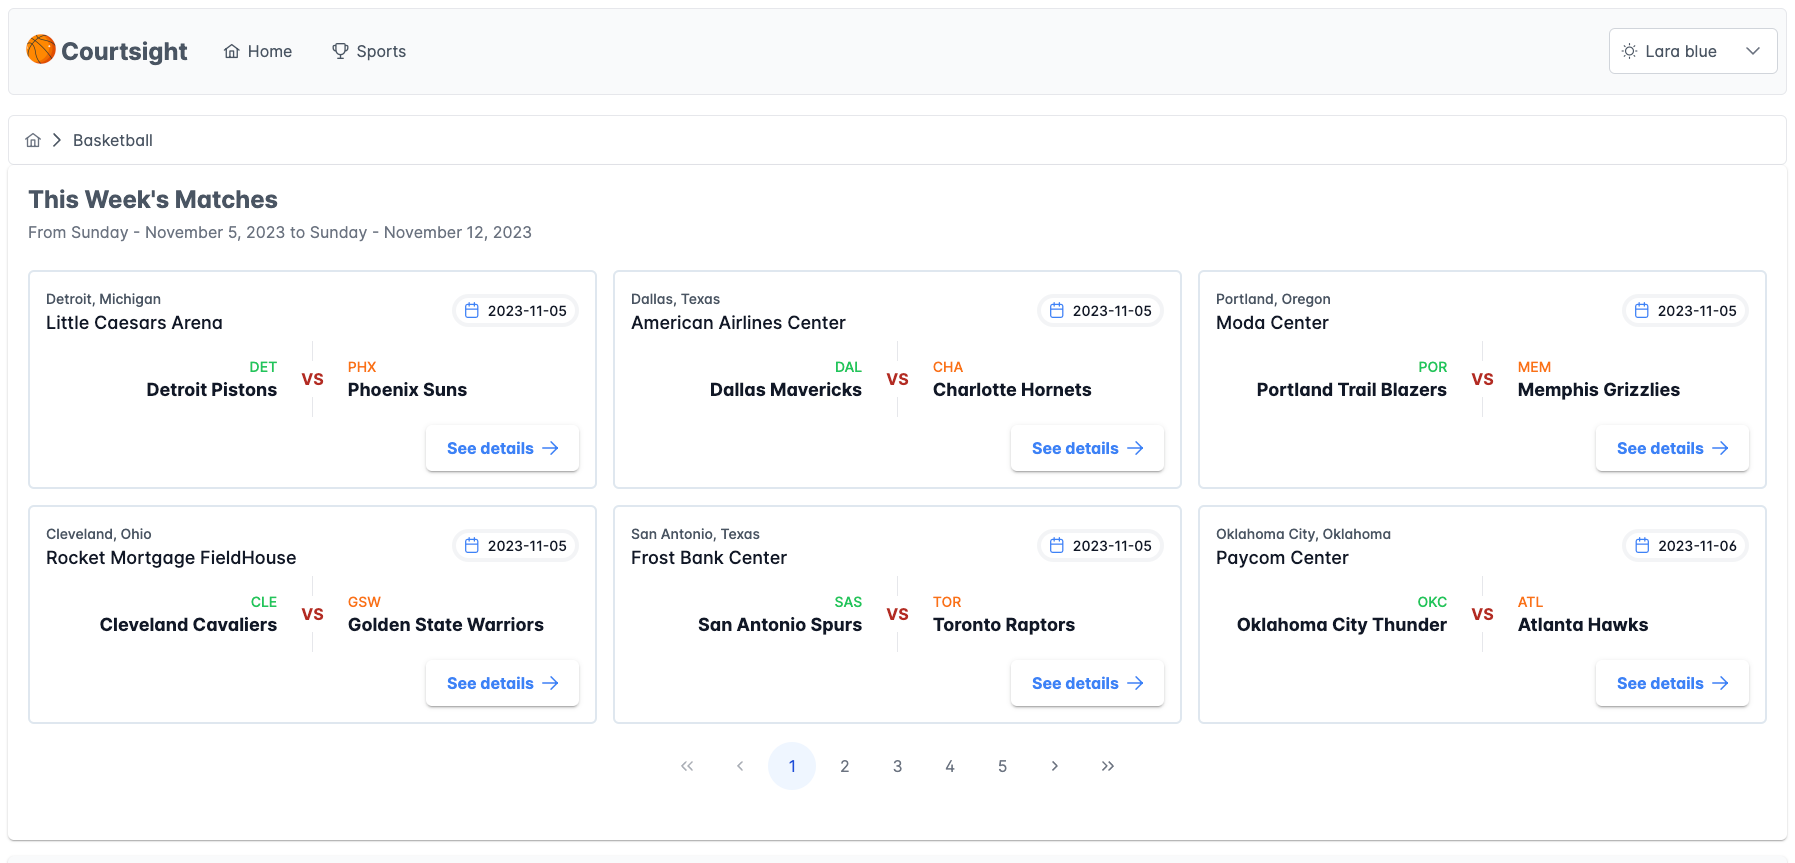
\includegraphics[width=0.75\linewidth]{img/webapp/basket_matches_list.png}}
        \caption{Lista dei prossimi match}
        \label{fig:enter-label}
    \end{figure}
    \begin{figure}[H]
        \centering
        \fbox{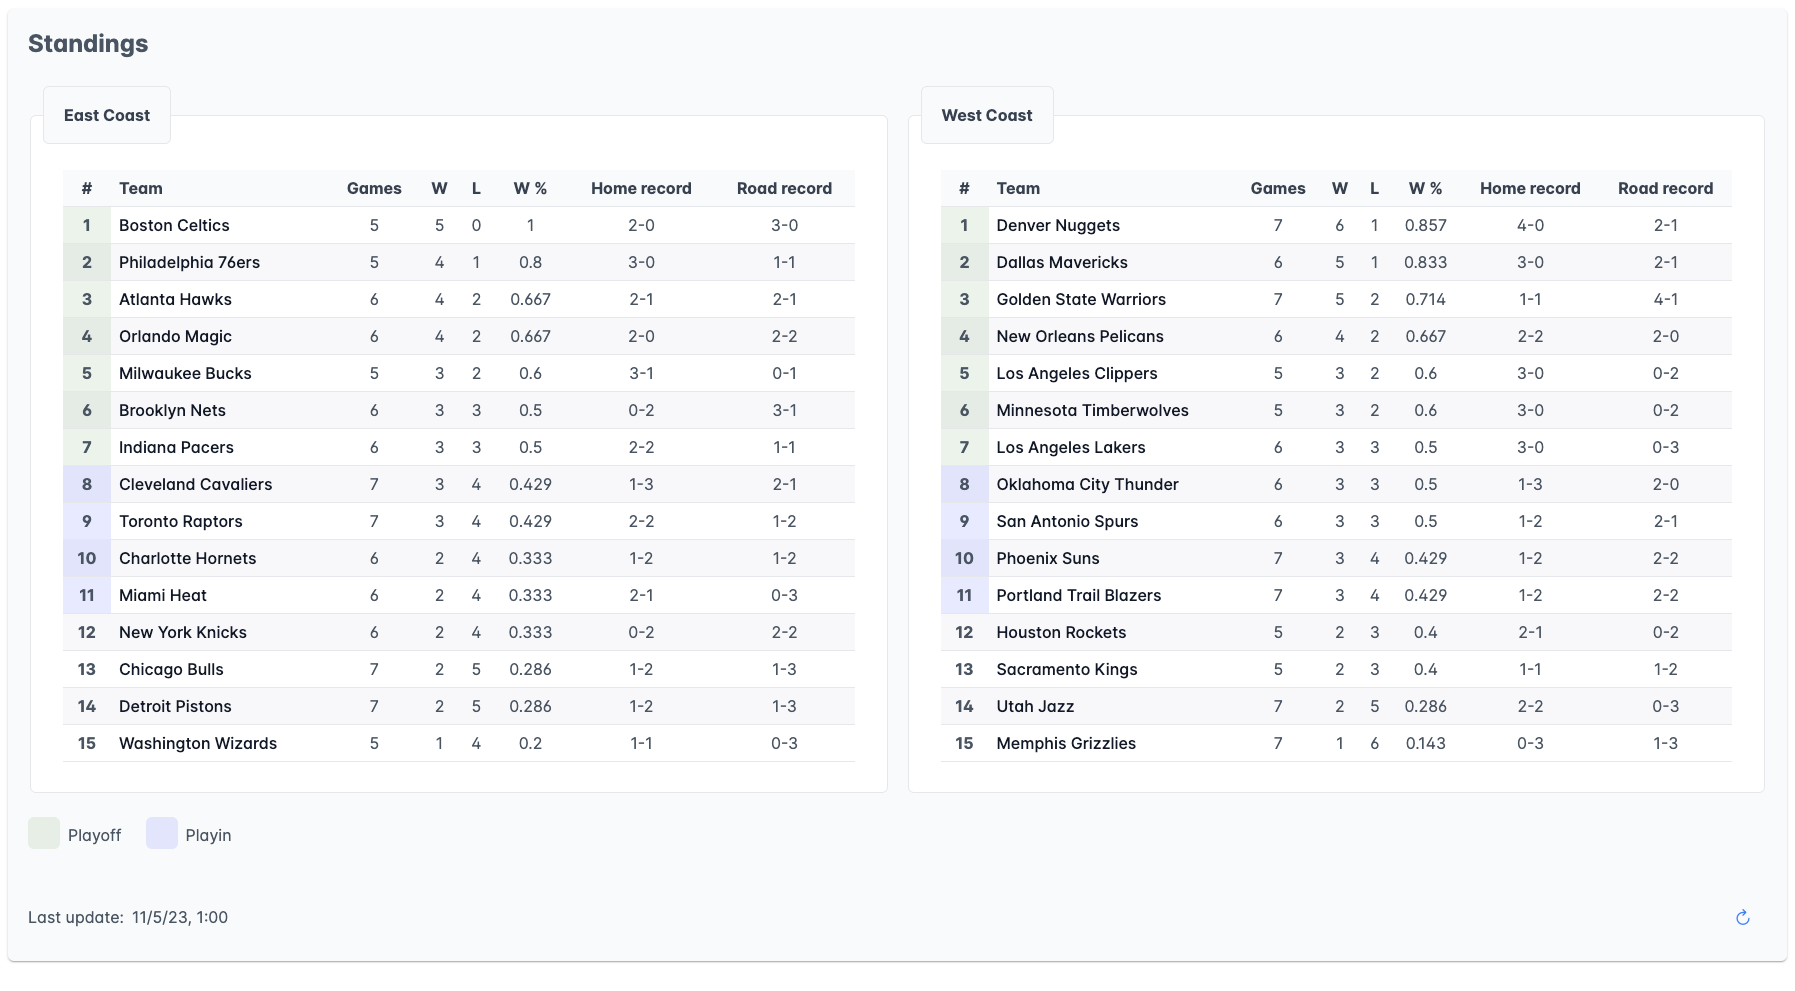
\includegraphics[width=0.75\linewidth]{img/webapp/basket_standings.png}}
        \caption{Classifica del campionato}
        \label{fig:enter-label}
    \end{figure}
    
    \paragraph{Basket - Squadra} Selezionando il nome di una squadra è possibile vedere i dettagli sulla sua data di fondazione e arena di casa, oltre all'elenco dei giocatori e le prossime partite che disputerà.
    \begin{figure}[H]
        \centering
        \fbox{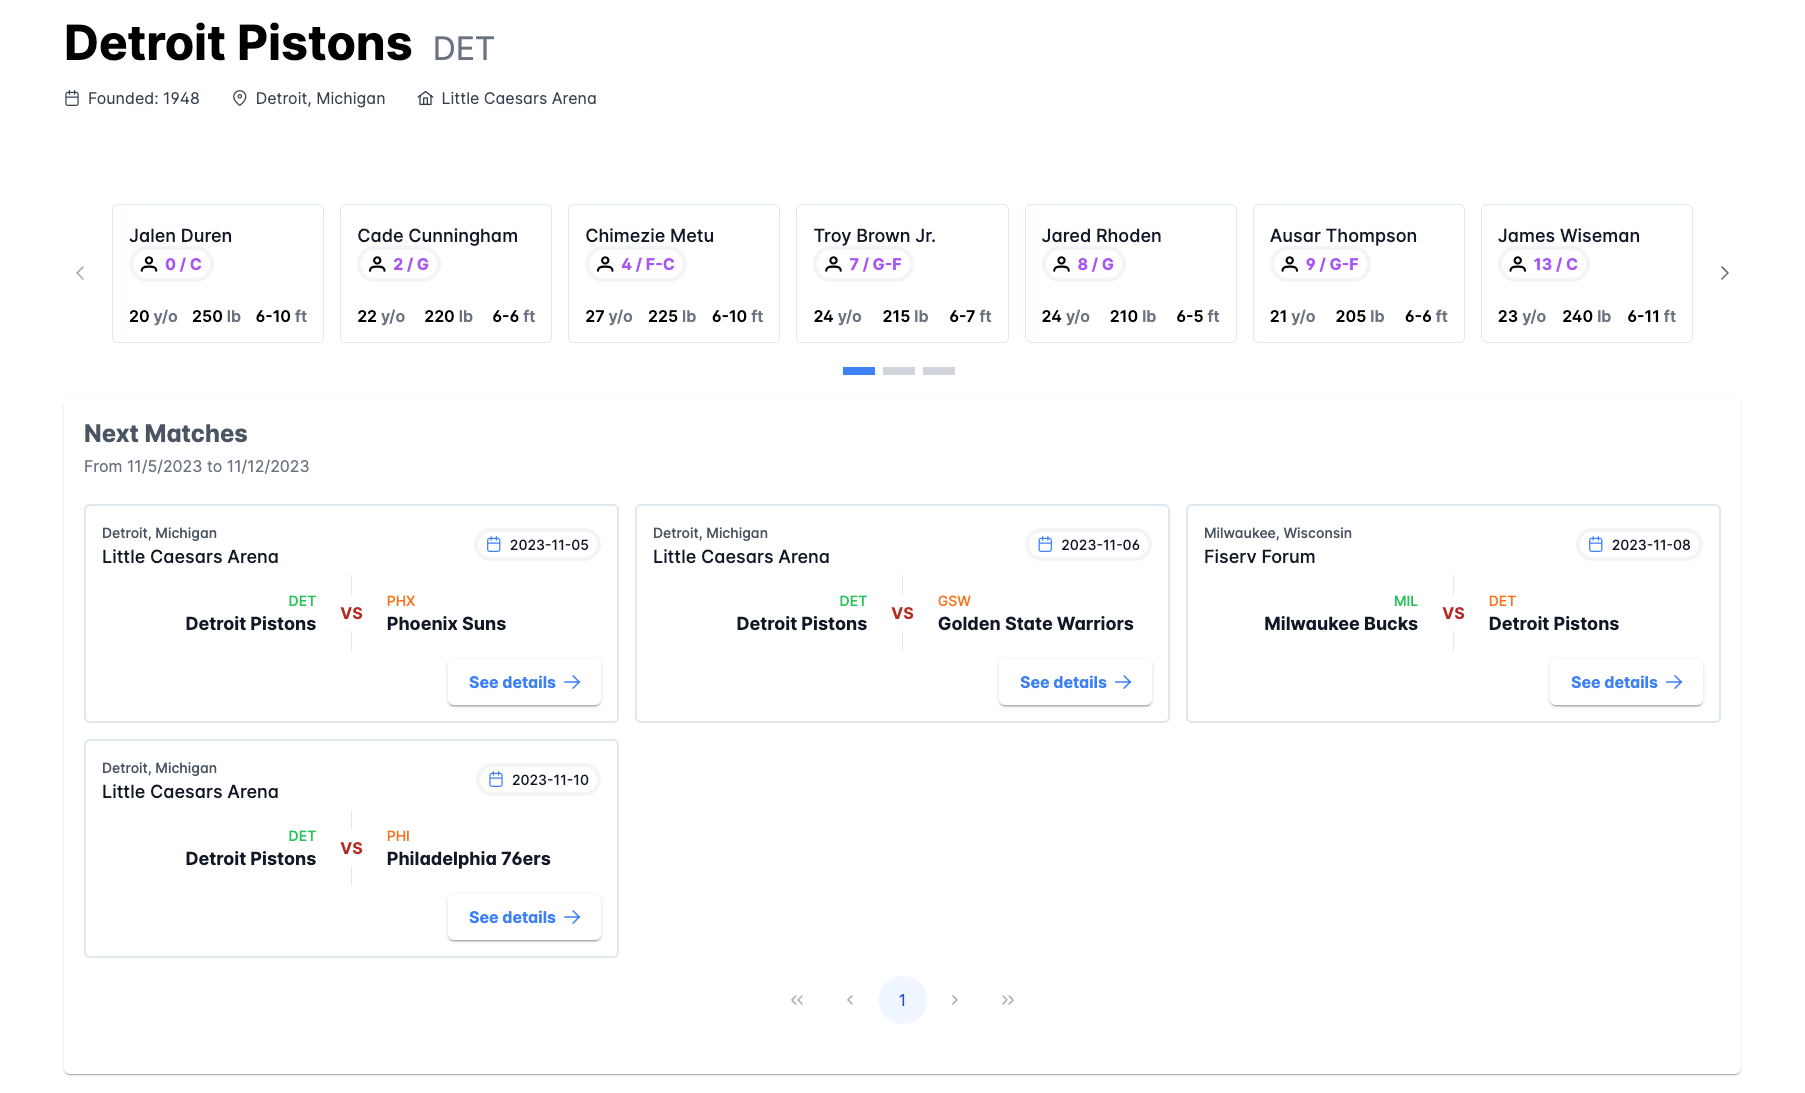
\includegraphics[width=0.75\linewidth]{img/webapp/team.png}}
        \caption{Dettagli squadra}
        \label{fig:enter-label}
    \end{figure}
    
    \paragraph{Basket - Partita} La schermata dedicata ai match è il vero luogo di incontro di tutti i microservizi sviluppati. Oltre a presentare il punteggio e le statistiche del match, è disponibile l'elenco di tutti i bookmaker e le quote della partita. Inoltre, premendo un bottone è possibile interrogare il modello di ML per predire il risultato del match.
    \begin{figure}[H]
        \centering
        \fbox{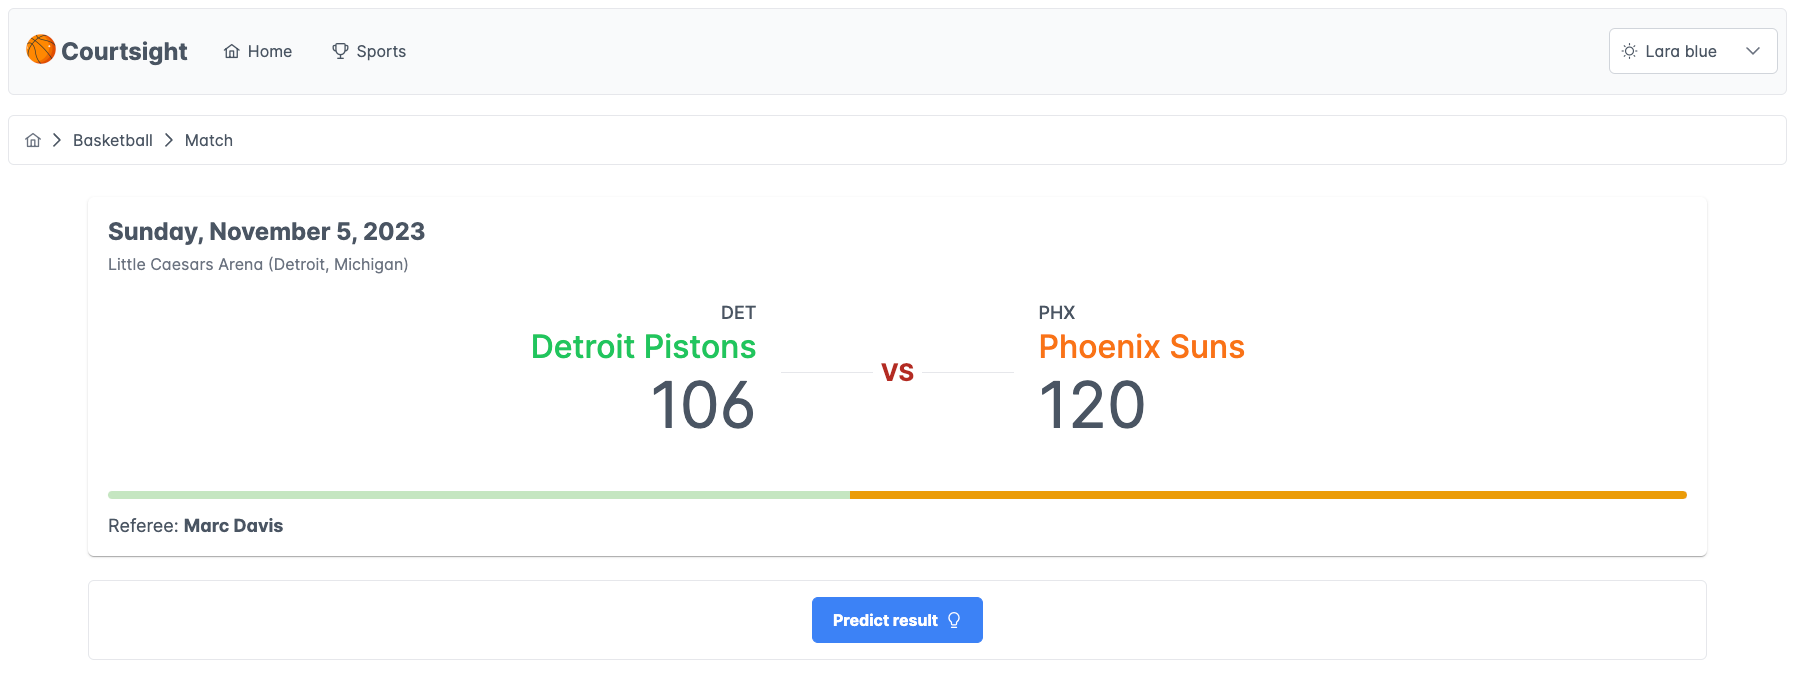
\includegraphics[width=0.75\linewidth]{img/webapp/match_header.png}}
        \caption{Informazioni match}
        \label{fig:enter-label}
    \end{figure}
    \begin{figure}[H]
        \centering
        \fbox{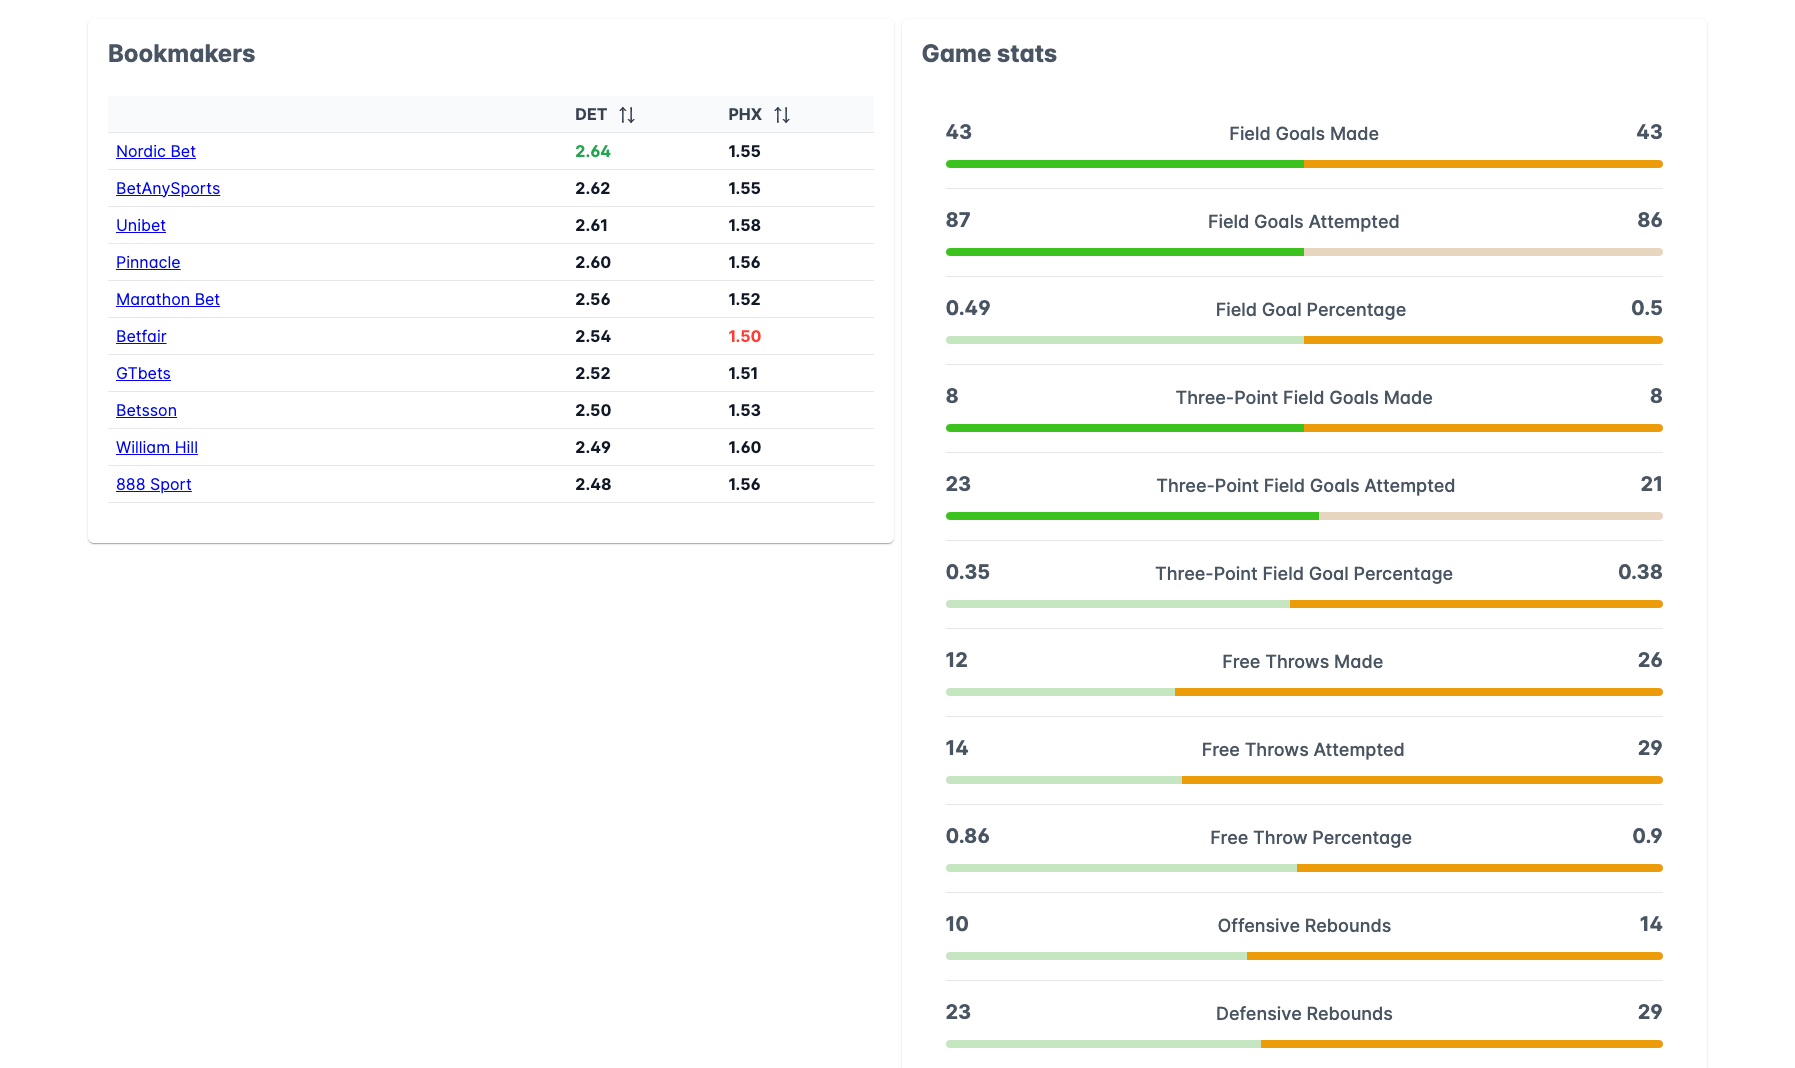
\includegraphics[width=0.75\linewidth]{img/webapp/match_stats.png}}
        \caption{Statistiche e quote match}
        \label{fig:enter-label}
    \end{figure}

Mediante il sistema di routing di Angular, le pagine sono definite ognuna da un diverso componente, inserito dinamicamente nel root della applicazione a seconda dell'url richiesto. 

\subsection{Struttura dell'applicazione}
In questa sezione verrà delineato l'intero elenco di componenti sviluppati. Nelle applicazioni Angular, quando il numero di componenti inizia a crescere, è bene suddividerli in cartelle organizzate per feature e l'elenco che segue presenta quindi la medesima strategia.

\subsubsection{app}
Alla base dell'applicazione web c'è un file \texttt{index.html} il cui body verrà dinamicamente aggiornato a runtime inserendo i vari componenti quando richiesto, e sarà quindi sempre presentato all'utente. 
\texttt{app-root} è l'unico componente indicato ed è il vero scheletro esterno dell'applicazione, in quanto verrà sempre disegnato. Ha al suo interno la barra del menu superiore, che ovviamente deve essere disponibile in ogni momento, e un contenitore fornito da Angular (\texttt{router-outlet}) per ospitare i componenti serviti dal sistema di routing. 
Il componente \texttt{menubar} oltre al titolo ospita anche i link ai vari sport e sulla sinistra un selettore del tema grafico da adottare, modificabile in tempo reale. 

\subsubsection{homepage}
L'homepage presenta semplicemente all'utente l'elenco degli sport disponibili. Questi sono ottenuti dinamicamente e mostrati a schermo in base alle feature disponibili. L'elenco degli sport e il singolo item sono quindi due componenti diversi, \texttt{sport-showcase} e \texttt{sport-details}, mostrati all'interno del macro componente \texttt{home}.

\subsubsection{basket/home}
La pagina principale dedicata all'NBA quando caricata effettua il \textit{fetch} delle partite della settimana che viene. Queste sono presentate come \texttt{match} all'interno di un elenco \texttt{match-list}, paginato a gruppi di sei. 

Subito sotto, la classifica aggiornata alla giornata corrente è resa disponibile dal componente \texttt{standings}. Questo, data la caratteristica del campionato di avere in realtà due classifiche in base alla costa (East Conference e West Conference), presenta due diverse tabelle \texttt{standings-list}. Oltre alla semplice posizione di ogni squadra sono anche forniti tutti i dati più rilevanti, come ad esempio partite vinte o record fuori casa.
Inoltre, le prime 8 righe di ogni tabella hanno una colorazione azzurra per segnalare che quelle squadre parteciperanno ai Playoff, mentre le successive 4 colorate di verde sono quelle che dovranno prima qualificarsi giocando i Play-in. 

\subsubsection{basket/team}
Ogni team ha una pagina dedicata, accessibile premendo sul suo nome ovunque compaia all'interno dell'app. Il componente \texttt{team-details} ospita, assieme a dettagli sulla squadra come anno di fondazione e arena di casa, l'elenco delle prossime partite da disputare (riutilizzando il componente \texttt{match-list}) e la lista di tutti i giocatori. Quest'ultimo componente (\texttt{players-showcase}) è un "carosello" che mostra di ogni giocatore ruolo, età, numero di maglia, peso e altezza.

\subsubsection{basket/match}
La schermata dedicata ai match ha in primo piano il risultato (corrente o passato) e dati quali data, palazzetto e arbitro. Due componenti sono poi disposti subito sotto. Il primo è \texttt{bookmakers-list}, che dati gli \textit{odds} di una partita mostra le quote per tutti i siti disponibili. Il secondo è invece \texttt{stats-table}, una lista di \texttt{stats-row} per elencare tutte le statistiche della partita (assist, rebound, falli, etc.).
Al centro della pagina un bottone permette, se premuto, di dare il via alle operazioni necessarie per predire il risultato della partita, ovvero recuperare il feature vector e inviarlo all'endpoint per ottenere infine lo score. Se questo risultato è disponibile, viene allora mostrato il nome del vincitore previsto del match e lo scarto di punti previsto. 

\subsubsection{\textit{time travel}}
Per permettere di visualizzare partite vere anche a campionato terminato, un semplice selettore di data è reso disponibile in fondo alle pagine dove sarebbe invece richiesta la data odierna. È possibile passare al componente una funzione di callback per essere notificati quando il cambiamento di data avviene. In questo modo è possibile gestire il reaload di tutti i componenti dopo aver effettutato un fetch dei nuovi dati.
\begin{figure}[H]
    \centering
    \fbox{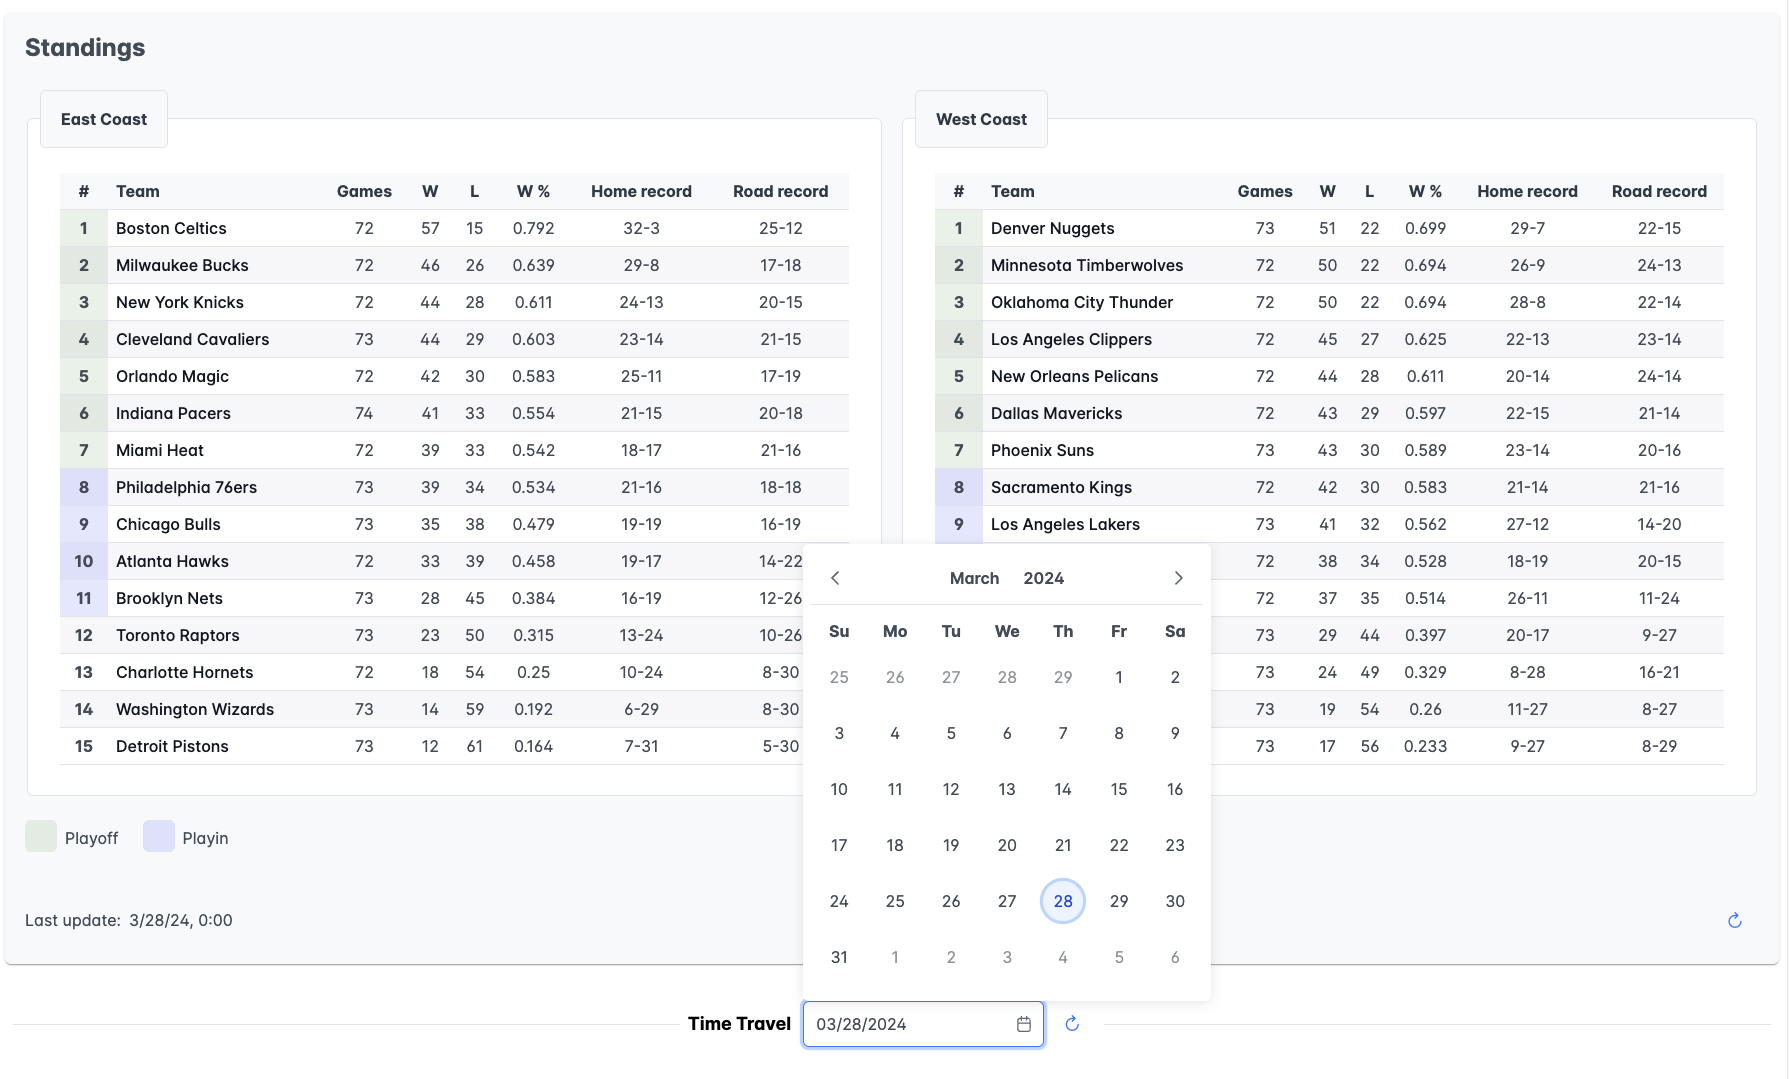
\includegraphics[width=0.75\linewidth]{img/webapp/timetravel.png}}
    \caption{Selezione data per "time travel"}
    \label{fig:enter-label}
\end{figure}


\subsection{Servizi}
Le applicazioni Angular sfruttano la Dependency Injection per rendere disponibili feature e dati ai vari componenti solo se esplicitamente richiesti. Una serie di \textit{services} sono definiti per interfacciarsi alle API e nascondere i dettagli in merito a chiamate e ottenimento dei dati.
I servizi sono divisi in file in base all'ambito di utilizzo anche se condividono in molti casi l'API a cui fanno riferimento. In particolare sono:
\begin{itemize}
    \item SportsService: ottiene dalla \texttt{bet\_api} l'elenco degli sport supportati.
    \item OddsService: ottiene dalla \texttt{bet\_api} le quote per un dato match.
    \item StandingsService: ottiene dalla \texttt{nba\_api} le classifiche aggiornate alla data richiesta.
    \item MatchesService: ottiene dalla \texttt{nba\_api} l'elenco delle partite in un intervallo di date, le statistiche relative a una data partita e il feature vector per un determinato incontro.
    \item TeamsService: ottiene dalla \texttt{nba\_api} informazioni generali relative a un team dato il suo "ticker" o le statistiche complete in base all'id.
    \item PlayersService: ottiene dalla \texttt{nba\_api} le statistiche di un dato giocatore.
    \item PredictionsService: ottiene dal modello di Machine Learning la previsione dello score dato un certo feature vector.
\end{itemize}
Tre ulteriori servizi sono definiti per mettere a disposizione dell'intera app impostazioni e feature condivise, ovvero:
\begin{itemize}
    \item TimeTravelService, per permettere di cambiare la data "odierna" di riferimento in tutta l'applicazione.
    \item BreadcrumbService, per la navigazione mediante breadcrumb.
    \item ThemeService, per il cambiamento dinamico del tema grafico.
\end{itemize}
\begin{figure}[H]
    \centering
    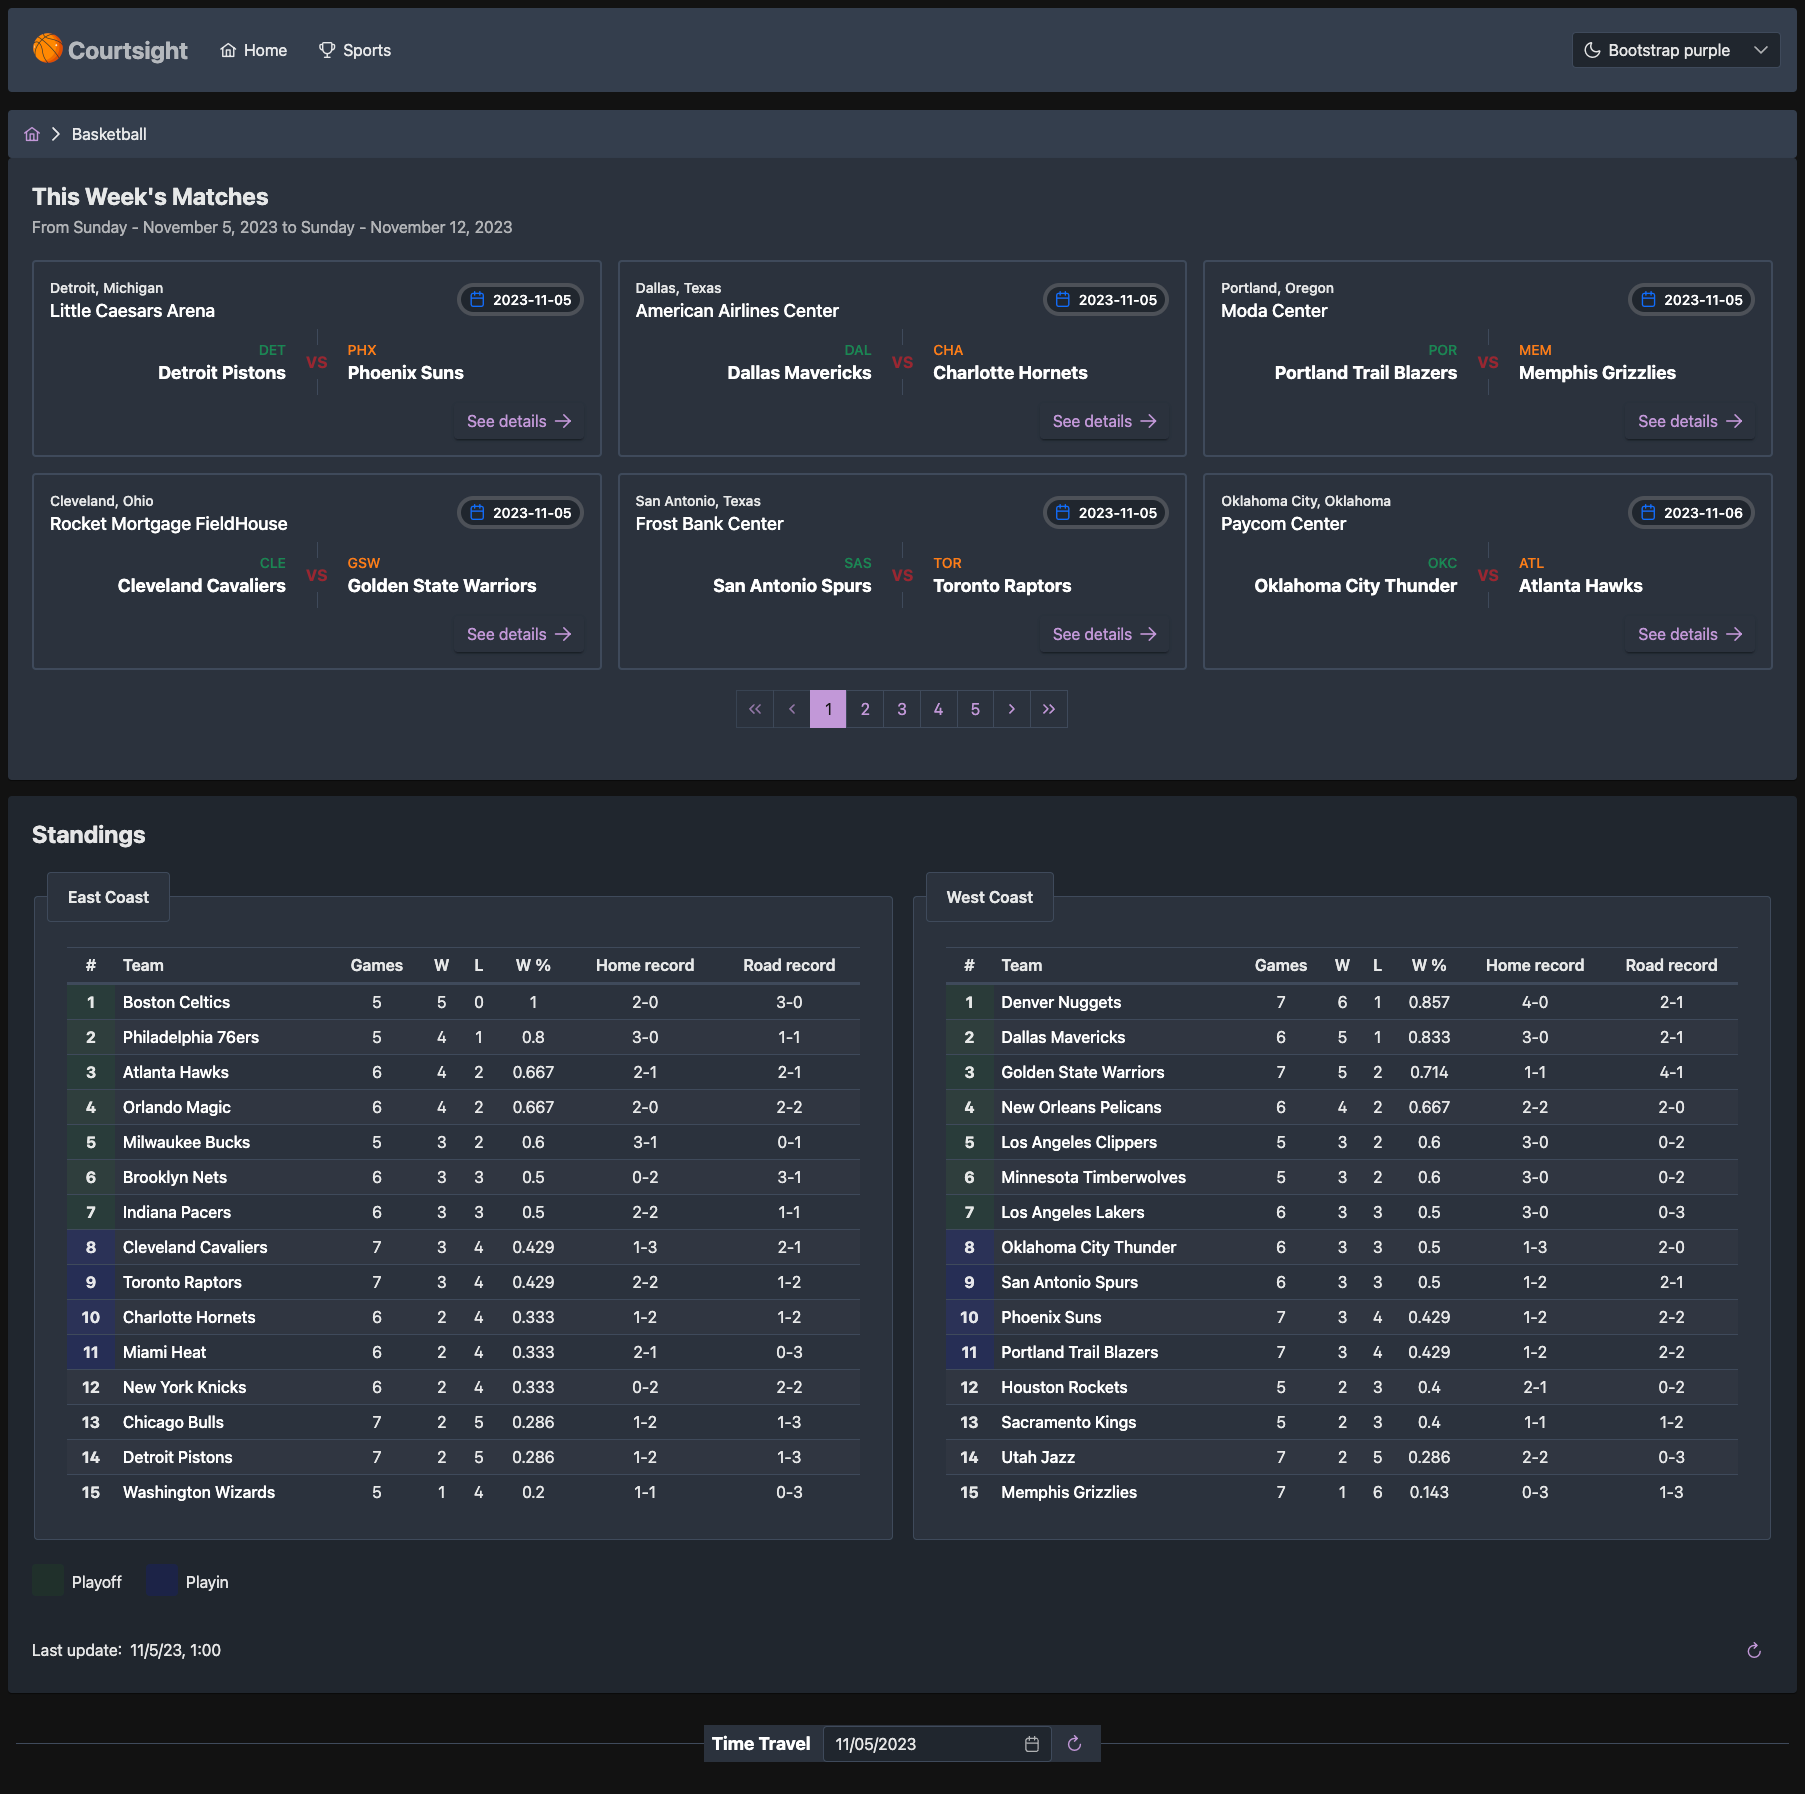
\includegraphics[width=0.75\linewidth]{img/webapp/themes.png}
    \caption{Dark mode selezionato dinamicamente}
    \label{fig:enter-label}
\end{figure}
\newpage
